\documentclass[12pt,a4paper]{article}
\usepackage{amsmath}
\usepackage{amsfonts}
\usepackage{amssymb}
\usepackage{makeidx}
\usepackage{graphicx}
\usepackage{listings}
\usepackage[hidelinks]{hyperref}
\usepackage[left=2cm,right=2cm,top=2cm,bottom=2cm]{geometry}
\author{Bet Peters - s1147919}
\title{Homework 4}

\begin{document}
\maketitle

\section{Duplicate detection}

Before I started this exercise, I rewrote (converted, mostly) my webcrawler to \texttt{C++ 11}. To cope with duplicates, I used an \texttt{unordered\_set}, which is an implementation of a hash set included in the default \texttt{C++} library, and a \texttt{queue}, also included by default.

In my hashset, I record which URLs are already included in the queue, so that I do not have to queue them again. When I take an entry from the queue, I also remove it from the set, so it no longer takes memory there.

When I queue a URL, I first check whether it already is in the queued set, and whether I have not already downloaded it. These are both very fast operations. If both are false, then I add the url to the queue and to the set of queued urls.

The advantage of using a hash set over using a binary tree, is that existence checking is of $O(1)$, rather than $O(\log n)$. This advantage is even greater when comparisons between elements are rather expensive, which string comparisons are.

A slight downside is that this way, every queued URL is stored in memory twice, once in the queued set. This is not too important, as the overall memory usage is still pretty low.

\section{Inverted index web searching}

I chose to do the medium difficulty exercise. To prepare, I recoded my current crawler to \texttt{C++ 11} to make full use of modern features. With the recode, I added a few features:
\begin{itemize}
	\item The crawler does some rate-limiting
	\item The crawler respects \texttt{robots.txt}
	\item The crawler can be stopped and started again, without causing duplicate entries in the index
	\item The crawler better respects redirects, and actually notices them
\end{itemize}
The crawler is entirely written by myself, except for the following external libraries:
\begin{itemize}
	\item cURL
	\item OpenSSL (for MD5 hashing)
	\item htmlstreamparser (included and slightly modified)\footnote{This is mostly limited to using \texttt{const char*} instead of \texttt{char*} in method signatures. This allowed for greater interoperability between \texttt{std::string} and the library.}
\end{itemize}
The inclusion of OpenSSL does not pose an additional dependency on the host system, as it was required for cURL anyway.

\subsection{Building the programs}

Due to the default compiler on the NUWD systems being not exactly new, the program will not compile. However, there is a more recent compiler available. To use it (and the program, one must first enter the following:\footnote{These instructions are for \texttt{bash} or \texttt{zsh}. Usage in other shells may differ slightly.}

\begin{lstlisting}[breaklines,numbers=left,language=bash]
source /vol/share/software/gcc/5.3.0-profile
export LD_LIBRARY_PATH="/vol/share/software/gcc/5.3.0/lib64:/vol/share/software/gcc/5.3.0/lib32:$LD_LIBRARY_PATH"
\end{lstlisting}
without the line break in the second line. This will instruct your shell to use the more recent version of gcc and the more recent libraries.

After doing so, the program can be built with \texttt{make} and run normally. Please note that the updated library export is needed for running the program, not just compiling. The webcrawler can be used with \texttt{./webspider [URL]}, where \texttt{[URL]} is a valid url including protocol. It will then do a modified breadth first search starting at that URL, skipping any pages already in the index.

Note that \texttt{make} creates all necessary directories for the indices. If you run the program in a different folder, make sure those directories exist.

\subsection{Being a nice bot}

For this exercise, I wanted my bot to crawl the entire internet, not just our local websites. To do this, I had to be nicer to sites than I have been until now.

First of all, need to limit my requests to a certain server within a given timespan, to avoid performing a Denial of Service attack. To do this, I record the last time I visited a domain for every domain I encounter, and if I consider a URL within 2 seconds of visiting another on the same domain, I send that URL to the back of the queue instead of crawling it.

I also need to somewhat respect \texttt{robots.txt} files. Since building a parser for the robots exclusion protocol was not within the scope of this assignment, I opted to only regard the \texttt{Disallow:} lines, and obey all of them, rather than the ones specific to my user agent. Some major websites (like Facebook and Wikipedia) have a robots.txt file disallowing all pages to some robots.

Finally, I changed my user agent string to include my umail email address, so that if anyone was harassed by my crawler, they could contact me. None have.

\subsection{Building reverse indices}

To build the reverse indices for the files, we need to have a file for every word and every url. Since those things can contain special characters, I opted to instead use the MD5 hash. Since OpenSSL was already an indirect dependency due to cURL, I used their implementation of the hashing algorithm rather than writing my own. I then used the hexadecimal representation of the hash as the filenames.

For fairness, I considered only the first occurrence of a word or link on a page\footnote{Some websites, like Youtube, link about 30 times on every page to the page itself.} to be added to the index.

It turns out, that this way of indexing is very slow on university computers, due to the network file systems not being that fast with opening and closing thousands of files. There is no real way around this, other than running the crawler on a local file system.

\subsection{Implementing keyword search}

The webquery system reads its keywords from a file \texttt{query.txt}, and only considers the first line of that file. This ensures that we have no arbitrary command execution when we call our query program.

To form our list of candidates, we

\begin{enumerate}
	\item Find all pages containing the keyword
	\item Give a page +1 relevance for containing the word in the page
	\item Give a page +4 relevance for containing the word in the title
	\item Give a page +16 relevance for containing the word in the url
	\item Give a page +1 for every page that links to it.
\end{enumerate}

All of these can be determined rather easily by finding the correct file (using MD5 hashes) and iterating over the lines. For multi-keyword searches, we do step 1-3 for every keyword separately, sum the weights (disregarding any page that does not occur in every set) and continue with that result.

After this, the results are sorted by relevance (descendingly) and printed to the standard output.

\subsection{Using the web interface}

The web interface is located in \texttt{index.php}. It needs a simple webserver to host it. I used the PHP builtin webserver, available from PHP 5.4 onward, but on university computers the mongoose server suffices.\footnote{The mongoose server is not included in the report due to licensing issues, but can be downloaded for free at \url{https://www.cesanta.com/products\#binary}}.\footnote{If possible, I recommend using the PHP builtin webserver, as Mongoose appears to have some issues with non-ascii characters.} Note that for Mongoose to properly work, a shebang (\texttt{\#!/usr/bin/php}) needs to be added to the top of the file. This is left out for compatibility with native PHP.

It takes a query from the URL (or the form) and writes it to \texttt{query.txt}, and then calls the \texttt{webquery} program.

To present a nice result to the user, I parse the original document as HTML, and show the user the first non-empty paragraph. This usually presents a nice snippet.

As a final touch, I named my search engine MIRgle, and copied the Google logo colours to my own. The final result can be seen in \autoref{fig:mirgle}. In my tests, I let my index build until I had about 12000 crawled pages.

\subsection{Image search}
I also implemented image search. Images are indexed based on the title of the page where they appear and their alt-text, if available.

I did not keep a list of any images searched, or even checked whether I could download the images, so there are unfortunately quite a few images that fail to load. This is unfortunate, but downloading them all would have increased the size of my local repository by a lot, and it is over 4 gigabytes already.

Like the normal web search, the image search supports multiple search terms, and has some nice previews. A screenshot cann be seen in \autoref{fig:image-mirgle}.

\begin{figure}
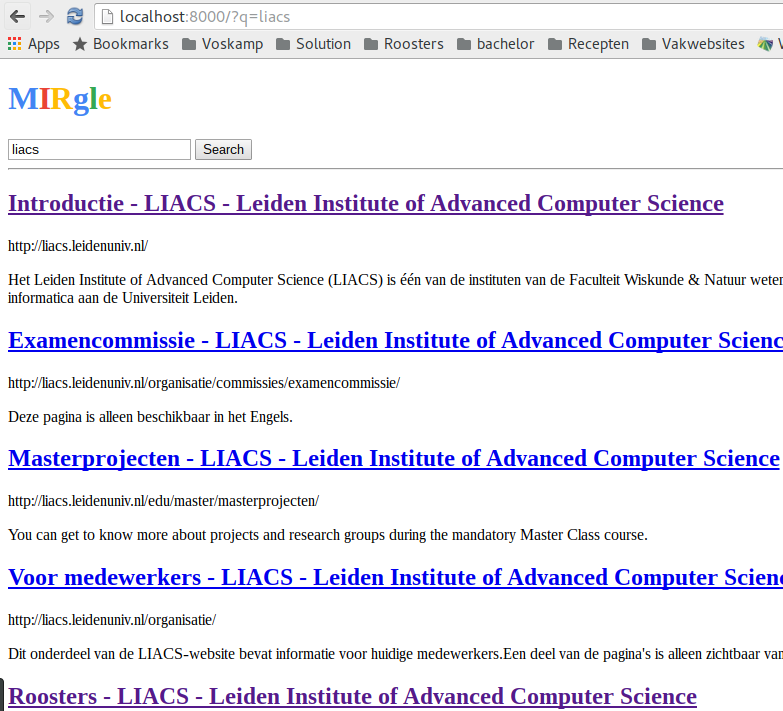
\includegraphics[width=\textwidth]{screenshot}
\caption{The results page of MIRgle}
\label{fig:mirgle}
\end{figure}

\begin{figure}
    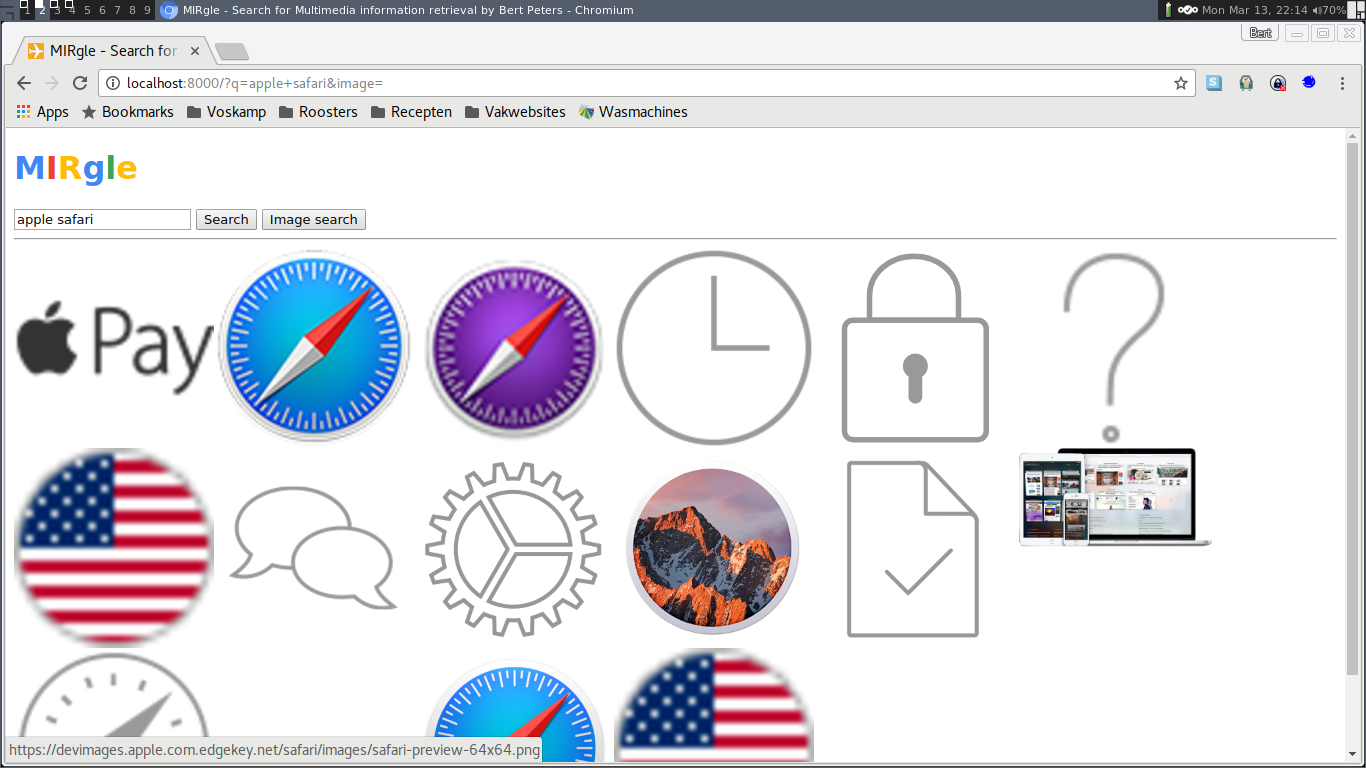
\includegraphics[width=\textwidth]{screenshot-img}
    \caption{The image results page of MIRgle}
    \label{fig:image-mirgle}
\end{figure}

\end{document}
